\section{Schaltung}
\label{sec:Schaltung}

\begin{figure}[!h]
	\centering
	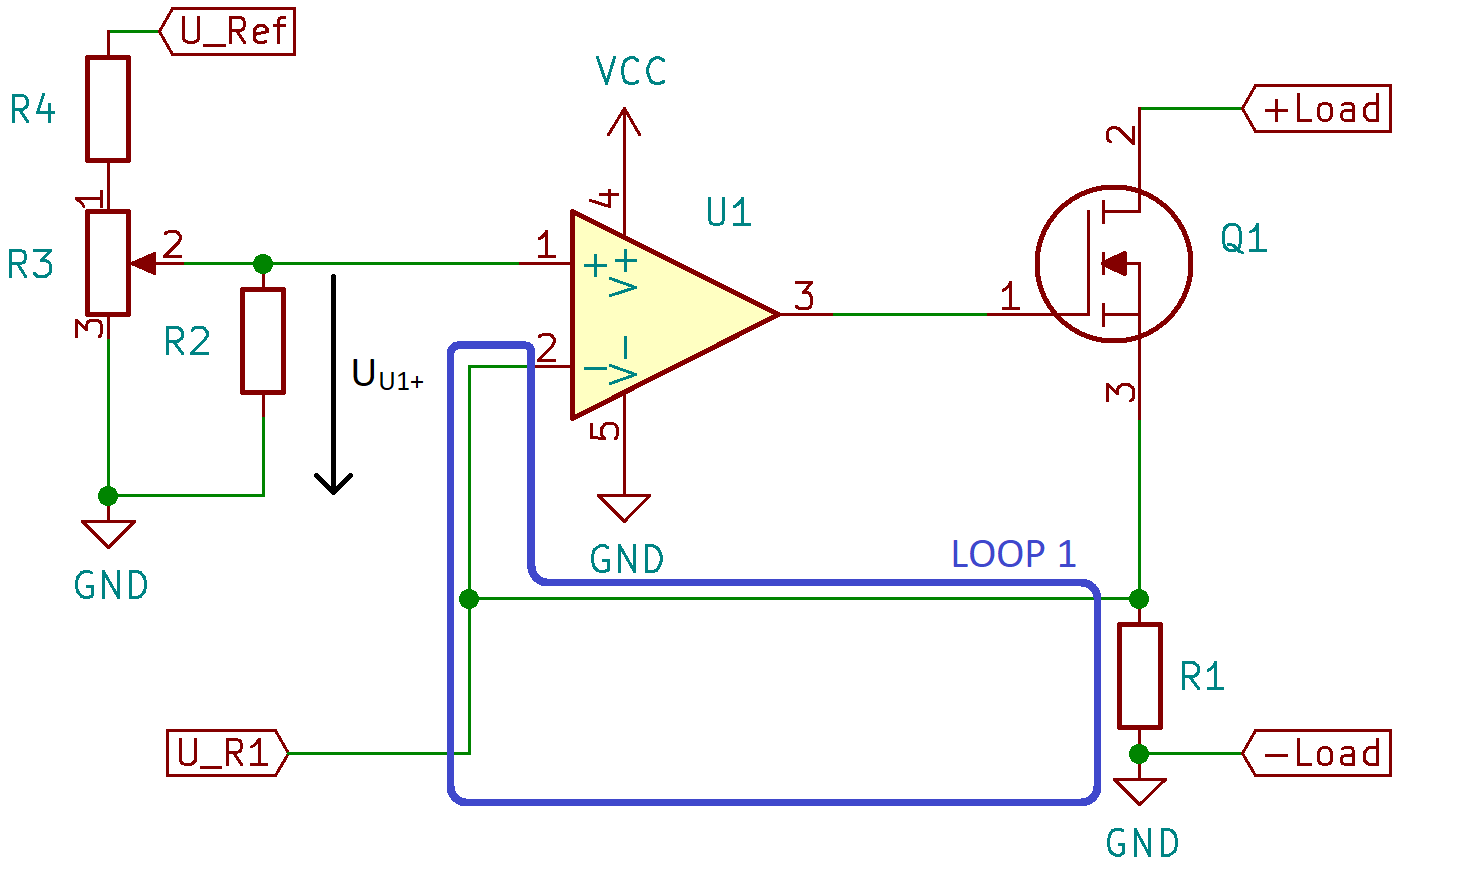
\includegraphics[width=0.5\textwidth]{Bilder/G_Schaltung.PNG}
	\renewcommand*\figurename{Schaltung}
	\caption{Grundschaltung}
	\label{sch:Grundschaltung}
\end{figure}

Die Grundlage dieser Schaltung geht auf die Shuntmessung und deren grundlegenden Zusammenhang von $U_{R1} = I_{R1} \cdot R1$ zurück.
Der N-Kanal MOSFET $Q_{1}$ wird bei dieser Schaltung im Widerstandsbereich betrieben und ist somit die einstellbare Last. 
Die elektrische Energie wird dort in Wärme umgewandelt.
Der Operationsverstärker (kurz OP) steuert sein Ausgangssignal so, dass am invertierenden (-) und nicht-invertierenden Eingang (+), 
keine Spannungsdifferenz herrscht.
Mit anderen Worten: Die Spannung über $R1$ ist gleich der Referenzspannung $U_{U1+}$ 
(einstellbarer Spannungsteiler mit $R2$, $R3$ und $R4$).
Somit ergibt sich der Zusammenhang von $I_{R1}$ und $U_{U1+}$ wie folgt:

\begin{equation}
	I_{R1} = \frac{U_{U1+}}{R1}
	\label{eq:IR1}
\end{equation}

In dem Spannungsteiler, der Referenz, ist bereits auf einen möglichen Fehlerfall und deren Folgen eingegangen.
Der Widerstand $R2$ verhindert, dass bei einem Kontaktproblem am Potentiometer die Spannung $U_{U1+}$ nicht undefiniert bleibt 
sondern auf GND Potential gelegt wird. 
Somit ist sichergestellt, dass die Last im Fehlerfall hochohmig geschaltet wird. 
Die Formel \ref{eq:UOp+} zu diesem Spannungsteiler beschreibt die Spannung am Eingang $U1+$. Unter anderem in Abhängigkeit des Winkels 
und des maximalen Winkels von dem Potentiometer $R3$.
Dabei ist $\alpha$ der Winkel zwischen Schleifer (Kontakt 2) und Kontakt 3.
Diese Formel kann für beide Anschläge zu den Formeln \ref{eq:UU1max_min} stark vereinfacht werden.
Die allgemeine Formel des Spannungsteilers lässt einen nahezu linearen Zusammenhang zwischen Spannung $U_{U1+}$ 
und Winkel $\alpha$ erkennen. Zur Berechnung des maximalen Stromes $I_{R1,max}$ genügt die Betrachtung der Spannung 
$U_{U1+,max}$ (Formel \ref{eq:UU1max_min}).

\begin{equation}
	U_{U1+} = U_{Ref} \cdot \frac{\frac{R2 \cdot R3 \cdot \frac{\alpha}{\alpha_{max}}}
									{R2 + \big(R3 \cdot \frac{\alpha}{\alpha_{max}}\big)}}
							{R4 + \frac{R2 \cdot R3 \cdot \frac{\alpha}{\alpha_{max}}}	
									{R2 + \big(R3 \cdot \frac{\alpha}{\alpha_{max}}\big)} + \Big(R3 \cdot 
									\frac{(\alpha_{max} - \alpha)}{\alpha_{max}} \Big)}
	\label{eq:UOp+}
\end{equation}
\vspace{0,1cm}
\begin{equation}
	U_{U1+,max} = U_{Ref} \cdot \frac{\frac{R2 \cdot R3}{R2 + R3}}
							{R4 + \frac{R2 \cdot R3}{R2 + R3}}
		\qquad		
	U_{U1+,min} = 0
	\label{eq:UU1max_min}
\end{equation}

\begin{figure}[!h]
	\centering
	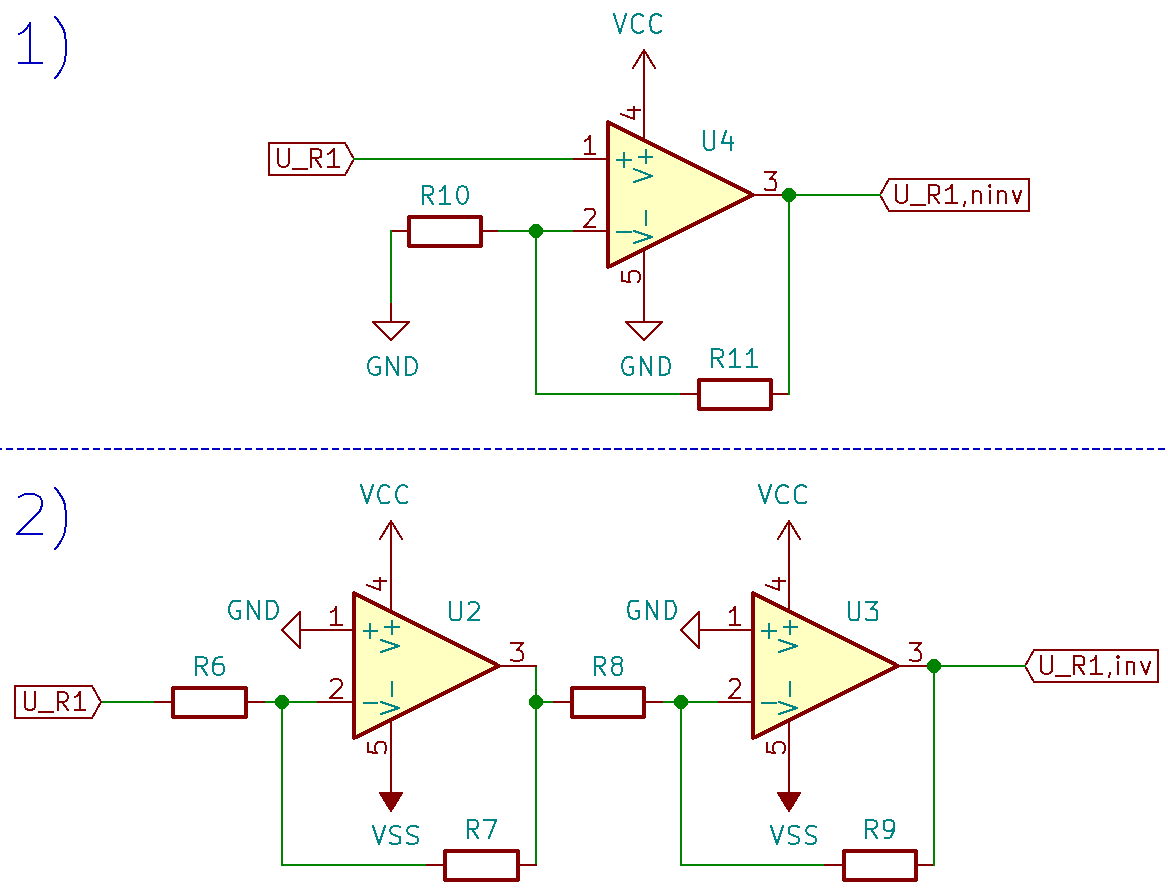
\includegraphics[width=0.45\textwidth]{Bilder/OP_Schaltung_analyse.PNG}
	\renewcommand*\figurename{Schaltung}
	\caption{Operationsverstärkerschaltungen zur Aufbereitung des Shuntsignals $U_{R1}$\\
		1) nicht-invertierender Verstärker\\
		2) zwei invertierende Verstärker }
	\label{sch:OP_Verstärkung}
\end{figure}

Damit der fließende Strom, mit beispielsweise einem Mikrocontroller, bestimmt werden kann, muss die Spannung $U_{R1}$ verstärkt werden. 
Dazu eignen sich zwei einfache Schaltungen.

Um kleine Spannungen mit Faktor größer 1,5 zu verstärken eignet sich die erste Schaltung. 
Die Schaltung des nicht-invertierenden Verstärkers (Schaltung. \ref{sch:OP_Verstärkung}.1) eignet sich daher für große Strombereiche bei 
relativ großem Shunt-Widerstand $R1$. 
Die Verstärkung ($V_{U4}$) berechnet sich nach:

\begin{equation}
	V_{U4} = 1+ \frac{R11}{R10}
	\label{eq:V_nichtInv}
\end{equation}

Zu erkennen ist, dass dieser Verstärker mathematisch keine $V$ $\leq 1$ realisiert werden kann.


In Schaltung Nr.2 sind zwei invertierende Verstärker hintereinander geschaltet. 
Diese ist für Strombereiche mit sehr großem Shunt-Widerstand $R1$ geeignet, da eine Verstärkung kleiner 1 
realisiert werden kann.
Die Verstärkung ($V_{ges}$) berechnet sich nach:

\begin{equation}
	V_{U2} = - \frac{R7}{R6}  
		\qquad
	V_{U3} = - \frac{R9}{R8}
	%\label{eq:V_Inv}
\end{equation}
\vspace{0cm}
\begin{equation}
	V_{ges} = V_{U2} \cdot V_{U3}
	\label{eq:V_Inv}
\end{equation}

Diese ist mit mehr Schaltungsaufwand verbunden, da aufgrund der Invertierung des Signals eine 
Bipolare-Spannungsversorgung nötig ist. 

